\subsection{BUF2PE}\label{BUF2PE}

BUF2PE is where the convolution computation is done, thus the cardinal module in the whole design. 

Its design is actually simple and elegant. A MAC unit MAC$yx$ is responsible for calculating the $(x, y)$ pixel in the output feature map\footnote{To be more precise, its relative position in the Pox$\times$ Poy block currently being processed}. Each unit is decoupled from one another, so no adder trees are required. 

\begin{figure}
    \centering
    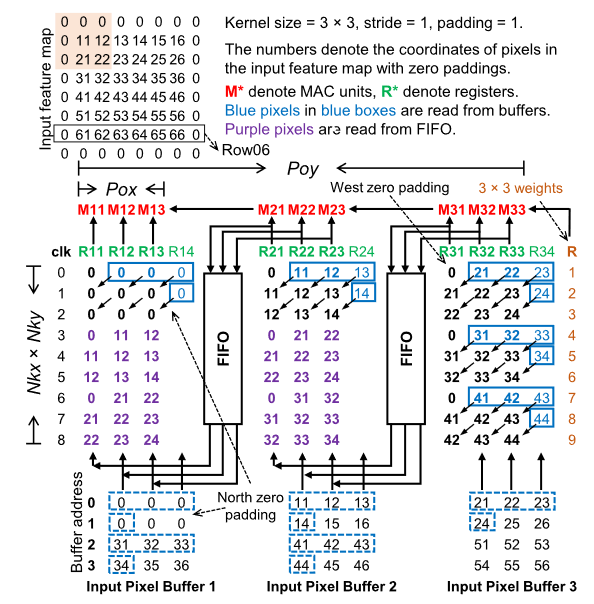
\includegraphics[width=0.8\columnwidth]{figures/BUF2PE.png}
    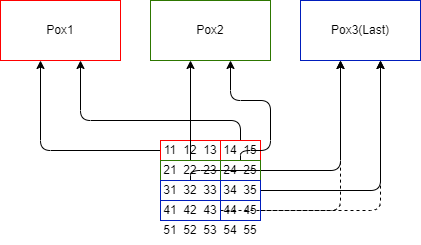
\includegraphics[width=0.8\columnwidth]{figures/act.png}
    \caption{BUF2PE and the mapping between activation data and PE}
\end{figure}

\begin{figure}
    \centering
    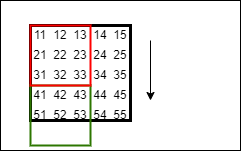
\includegraphics[width=0.8\columnwidth]{figures/task.png}
    \caption{The current region of output pixels to be produced(in red), the loaded data in buffer(in black), and the next region to be computed(in green)}
\end{figure}


We define \textit{Pox} as a compound of multiple \textit{MACs} which calculates the output pixels in the same row, and \textit{Poy} as a compound of multiple \textit{Pox}. So within the \textit{Pox}, each \textit{MAC} and its neighbour are using neighbouring pixels in the same row of the input map. Hence for one \textit{MAC}, its stream of input can be constructed from that of other \textit{MACs} by offsetting the time cycles. Similarly within the \textit{Poy} the neighbouring \textit{Poxes} are using neighbouring rows. This observation is crucial because it gives us a insight on how the data reuse can be done.

\paragraph{ For cycle $0 \to kernel\_size-1$} All MACs are first initialized with their corresponding rows read from buffer. Then the pixels are all shifted to the MAC to the left. From the observation above, we know the new pixels are exactly the new input required. A history of the input pixels are pushed into a FIFO for each \textit{Pox}.
\paragraph{ For cycle $kernel\_size \to kernel\_size * kernel\_size - 1$} The last \textit{Pox} continues its practice, while for the rest, their input can be sourced from their neighbouring \textit{Pox}. And so we do. We pop the data from the FIFO and take it as the new input for the remainder of \textit{Pox}.


In the implementation, for each \textit{MAC} a Mux is employed to decided from where a new pixel is fetched. As demonstrated, there can be three choice: \textbf{BUFFER}, \textbf{SHIFT} and \textbf{FIFO}. The state of the Mux is given according to the current row and column, and we use two interdependent counters to obtain them. Aligning the time series is the most tedious work during the design as a result.